\chapter{MEANIE/FIRE} 
\label{sec:meanie_fire}
\lstset{style=6502Style}

Since not all enemy formations use all six available slots for constituent meanies, any
spare slot can be employed to fire a bullet from one of the formation meembers.
Like the uridimine, the decision to launch is random but with a slight bias towards
greater frequency. It might not be obvious at first, but some attention has been paid
to ensuring that the bullets fired are appropriate for the meanie firing them. This is
assured by a little array, \fcode{bulletsForMeanies}, that at first might look a little
inscrutable.

\begin{lstlisting}[basicstyle=\scriptsize\ttfamily]
bulletsForMeanies
  .BYTE $0D,$12,$0D,$0C,$12,$0D,$0E,$0D ; A list of bullet types. The meanie's sprite
  .BYTE $10,$0F,$0C,$0C,$0E,$0D,$0D,$0C	; value is used to index into this list.
\end{lstlisting}

Each entry in this list gives the sprite for a type of meanie. It contains 16 entries,
and as you may recall, we have 16 different types of meanies. This means that selecting
the appropriate bullet is as simple as using the sprite value for our meanie as a lookup
value into the list. For example the first bullet in the list is for the meanie with a sprite
value of \icode{\$00}, the second is for the meanie with a sprite value of \icode{\$01}, and so
on. We get a clearer sense of this by putting the meanies and bullets together below.

\begin{figure}[H]
  \centering
  \begin{adjustbox}{width=10.0cm,center}
    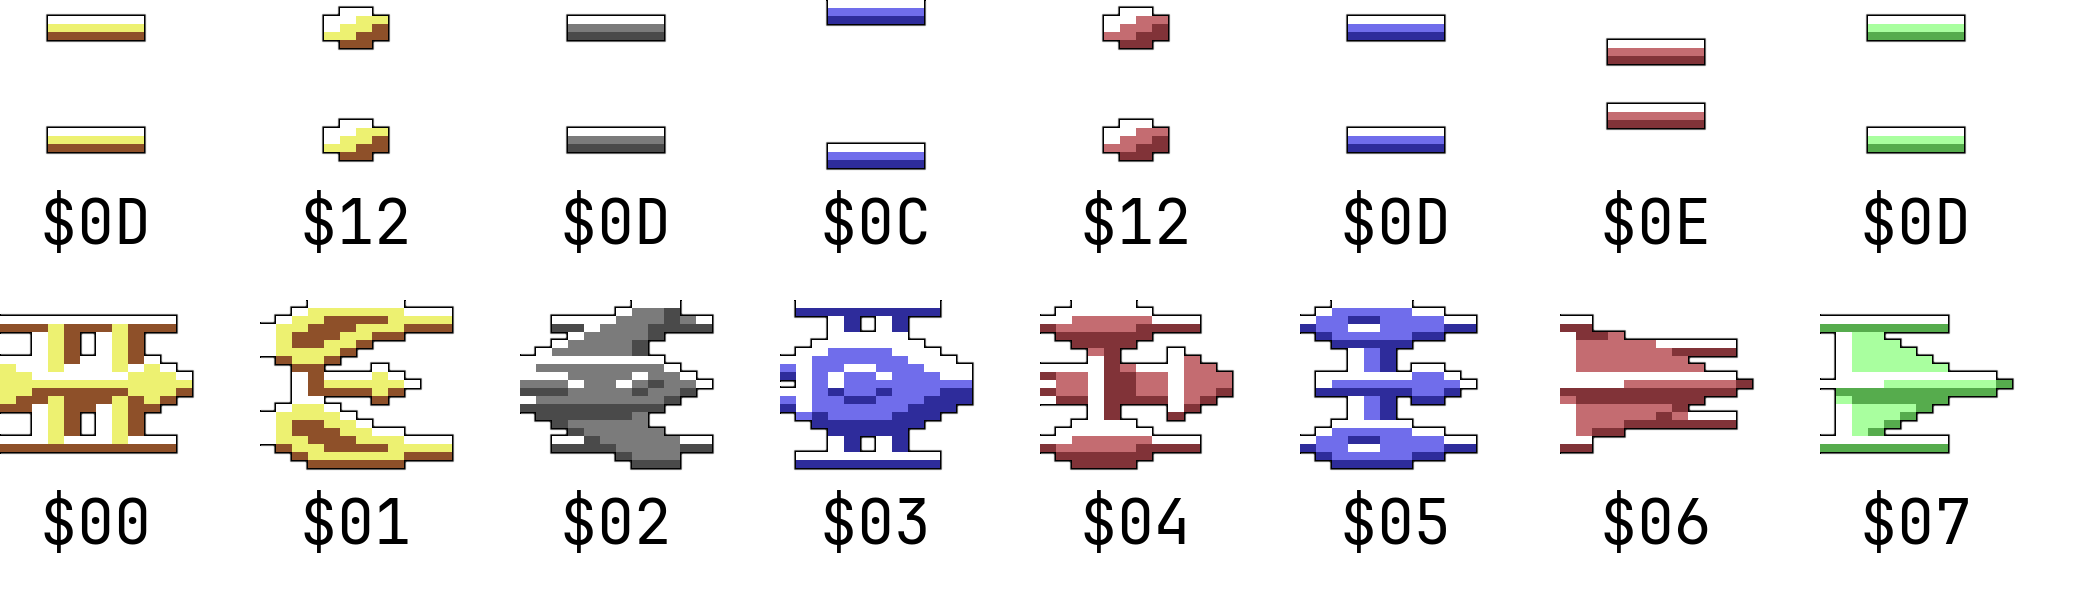
\includegraphics{src/enemy_bullets/bullet_array_0.png}%
  \end{adjustbox}
\end{figure}
\vspace{-0.4cm}
Notice how each bullet type aligns nicely with the position of the meanie's cannons. Below we have
two entries where the enemy has no obvious firing accoutrement, in those cases we just have a single
bullet that will emanate from its centre.
\begin{figure}[H]
  \centering
  \begin{adjustbox}{width=10.0cm,center}
    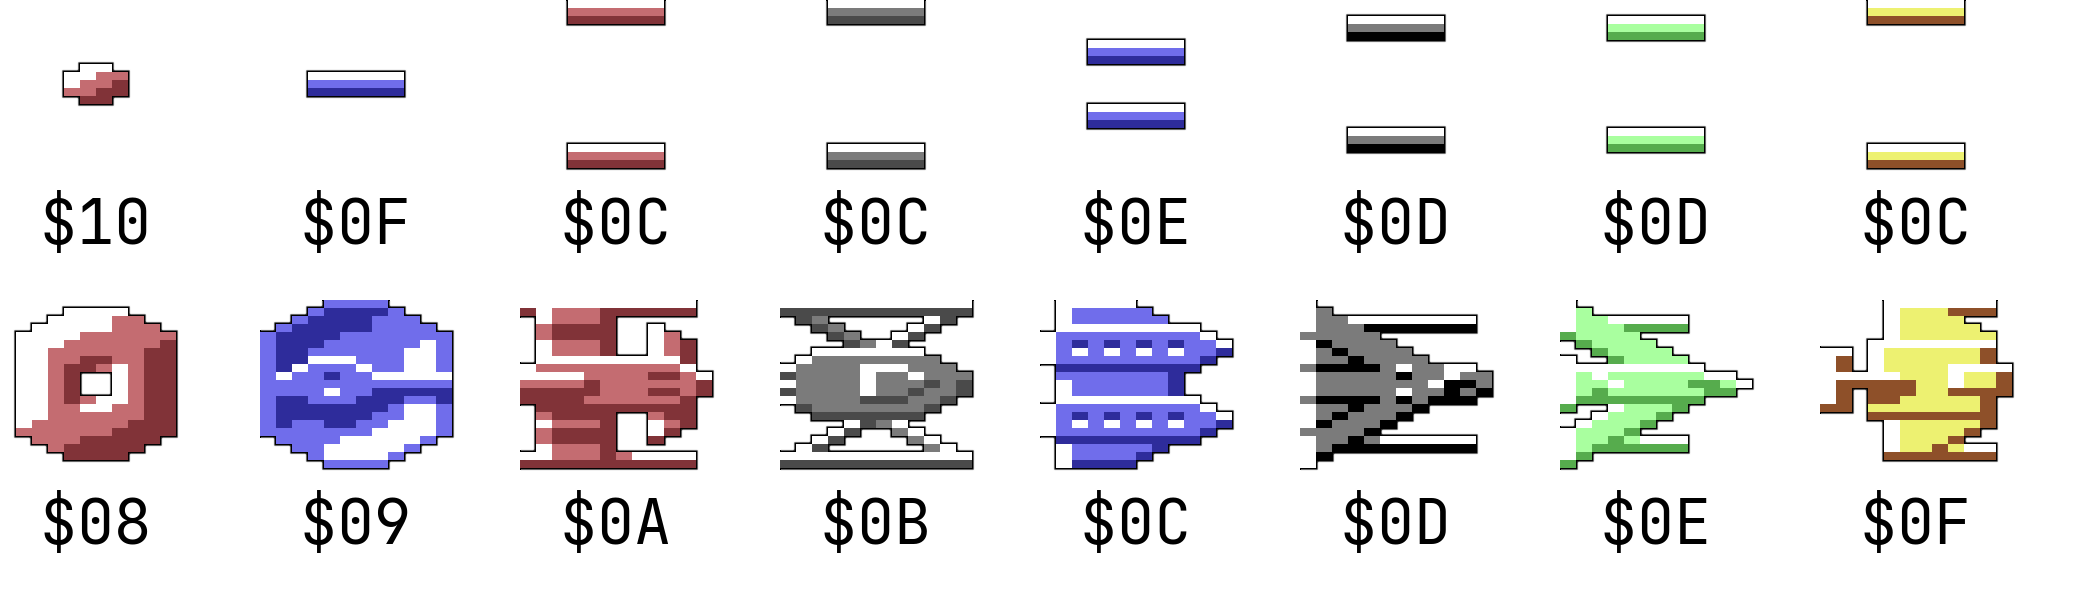
\includegraphics{src/enemy_bullets/bullet_array_1.png}%
  \end{adjustbox}
\end{figure}
\vspace{-0.4cm}

The full lifecycle of a bullet is similar to the one we explored for a uridimine. Once we've identified
a firing opportunity, our first task is to find a free slot for the bullet. We iterate through all six
slots and if one is lying vacant we take our chance and call \fcode{FireEnemyBullet}.

\vspace{-0.2cm}
\begin{minipage}[c]{0.30\linewidth}
	\vspace{-0.1cm}
	\begin{figure}[H]
		\centering
		\begin{adjustbox}{width=4.0cm,center}
			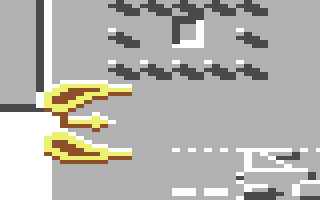
\includegraphics{src/enemy_bullets/level9_maybe_fire_bullet.png}%
		\end{adjustbox}
	\end{figure}
\end{minipage}
\begin{minipage}[c]{0.68\linewidth}
\begin{lstlisting}[basicstyle=\scriptsize\ttfamily]
MaybeFireEnemyBullet
  LDY #$05            ; Check all six slots.
FindAFreeSlot   
  LDA indexToEnemyUpdatePtrArray,Y ; Check the slot.
  BEQ FireEnemyBullet ; If it's free, fire a bullet.
  DEY                 ; Otherwise, check next slot.
  BPL FindAFreeSlot   ; Keep looping through all slots.
  RTS
\end{lstlisting}
\end{minipage}

\fcode{FireEnemyBullet} below takes care of loading and displaying the bullet
sprite. Notice how it displays the bullet superimposed on the enemy, you have
to look closely at the illustration below to see that the bullet has appeared
over the enemy's body. This happens only
briefly and is barely observable, as control is quickly passed to
\fcode{AnimateEnemyBullet}. 


\vspace{-0.2cm}
\begin{minipage}[c]{0.30\linewidth}
	\vspace{-0.1cm}
	\begin{figure}[H]
		\centering
		\begin{adjustbox}{width=4.0cm,center}
			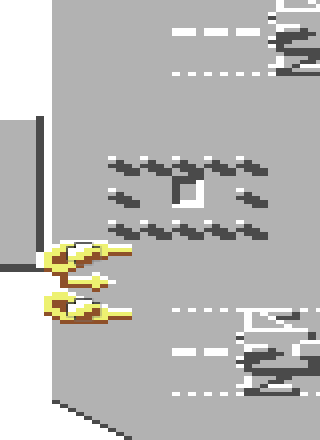
\includegraphics{src/enemy_bullets/level9_fire_bullet.png}%
		\end{adjustbox}
	\end{figure}
\end{minipage}
\begin{minipage}[c]{0.68\linewidth}
\begin{lstlisting}[basicstyle=\scriptsize\ttfamily]
FireEnemyBullet
  STY spriteIndex          ; Store our slot number.
  LDA currentSpriteValue   ; Stash the current sprite..
  PHA                      ; .. on the stack.
  LDA #$FF                 ; Turn off sprites..
  STA spriteEnable         ; .. for now.
  LDA bulletSprite         ; Get selected bullet sprite
  STA currentSpriteValue   ; and store it as our sprite.
  JSR DisplayCurrentSprite ; Display it.
  LDA #$04                 ; Let AnimateEnemyBullet take..
  STA indexToEnemyUpdatePtrArray,Y ; ..over.
  LDA #$A0                ; Set the duration of the ..
  STA movementDuration,Y  ; ..bullet's lifetime.
  PLA                     ; Get old sprite from stack.
  STA currentSpriteValue  ; And put in current sprite.
  INC bulletsInProgress   ; Flag bullet as active.
  LDY stashedYValue       ; Restore the old..
  STY spriteIndex         ; ..sprite index.
  RTS
\end{lstlisting}
\end{minipage}
Notice how \fcode{FireEnemyBullet} has to be careful about keeping the sprite value for the enemy
that fired the bullet on file. It does this by stashing the enemy's \fcode{currentSpriteValue} on the
stack (\fcode{PHA}) and then, once the bullet has been set up, restoring it to \fcode{current\-Sprite\-Value}
again with \fcode{PLA}. This \fcode{PHA}/\fcode{PLA} combination is an assembly-language pattern for stashing
away the current value of the \icode{A} register when we need to use the \icode{A} register for something else.

Moving on, \fcode{AnimateEnemyBullet} manages the active life of the bullet as it travels horizontally
across the screen. By design, it will travel in the same direction as the enemy that fired it.
\fcode{AnimateEnemyBullet} will also detect collision with the player's manta, but like the uridimine, only
if the manta is at cruising altitude. This check is cleverly performed by using the position of the
manta's shadow - if the offset for the shadow is greater than 20 pixels then the player has succesfully
avoided collision by maneuvering to a higher altitude.

If it doesn't manage to strike its target, the bullet will run out of time. When that happens we call
\fcode{BulletExpired}.

\vspace{-0.2cm}
\begin{minipage}[c]{0.30\linewidth}
	\vspace{-0.1cm}
	\begin{figure}[H]
		\centering
		\begin{adjustbox}{width=4.0cm,center}
			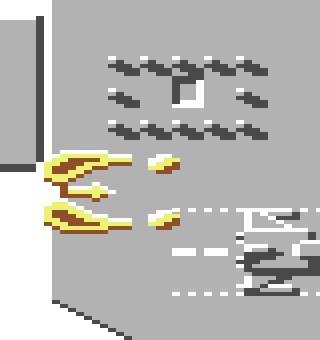
\includegraphics{src/enemy_bullets/level9_animate_bullet.png}%
		\end{adjustbox}
	\end{figure}
\end{minipage}
\begin{minipage}[c]{0.68\linewidth}
\begin{lstlisting}[basicstyle=\scriptsize\ttfamily]
AnimateEnemyBullet
  JSR FollowMantaOnX         ; Follow Manta along X axis.
  JSR UpdateEnemySpriteXYPos ; Update new position.
  LDA movementDuration,Y     ; Update duration..
  SBC #$01                   ; .. by subtracting 1.
  STA movementDuration,Y     ; If we've reached zero..
  BEQ BulletExpired          ; .. the bullet has expired.
  JSR DetectHittingManta     ; Have we hit the manta?
  BCC DetectLeavingScreen    ; No, check if left screen.
  LDA mantaShadowOffset      ; Check player altitude.. 
  CMP #20                    ; On same level as bullet?
  BCS DetectLeavingScreen    ; No, check if left screen.
  INC hasMantaBeenHit        ; Yes, flag manta as hit.
  JMP DetectLeavingScreen    ; Check if left screen.
\end{lstlisting}
\end{minipage}

A bullet visibly expiring on screen is a rare event, usually they either hit their target
or disappear out of sight. But on the off-chance that they are visible when their time is up
we set in train a little explosion. The bullet sprite is replaced with the initial sprite for
an enemy explosion (\icode{\$14}) and control is passed to \fcode{AnimateEnemyExplosion}. 

\vspace{-0.2cm}
\begin{minipage}[c]{0.30\linewidth}
	\vspace{-0.1cm}
	\begin{figure}[H]
		\centering
		\begin{adjustbox}{width=4.0cm,center}
			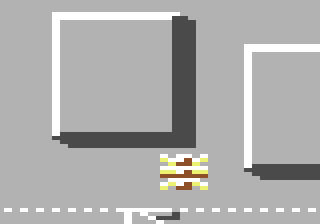
\includegraphics{src/enemy_bullets/level9_bullet_expired.png}%
		\end{adjustbox}
	\end{figure}
\end{minipage}
\begin{minipage}[c]{0.68\linewidth}
\begin{lstlisting}[basicstyle=\scriptsize\ttfamily]
BulletExpired
  LDA #$14               ; Get the explosion sprite.
  STA currentSpriteValue ; Store it as current sprite.
  LDA #$06               ; Make AnimateEnemyExplosion..
  STA indexToEnemyUpdatePtrArray,Y ; ..take over.
  LDA #$0A               ; Get an explosion sound.
  STA soundVariable      ; And play it later.
  JMP DetectSpriteLeavingScreen ; Check leaving screen.
  ; Returns
\end{lstlisting}
\end{minipage}

We have already encountered \fcode{AnimateEnemyExplosion} in our section on the uridimine.
The routine for managing the explosion of uridimines is also used for managing the explosion
of bullets. We can see the full sequence below, starting at sprite \icode{\$14} and finishing
at sprite \icode{\$1D}.

\begin{figure}[H]
  \centering
  \begin{adjustbox}{width=12.0cm,center}
    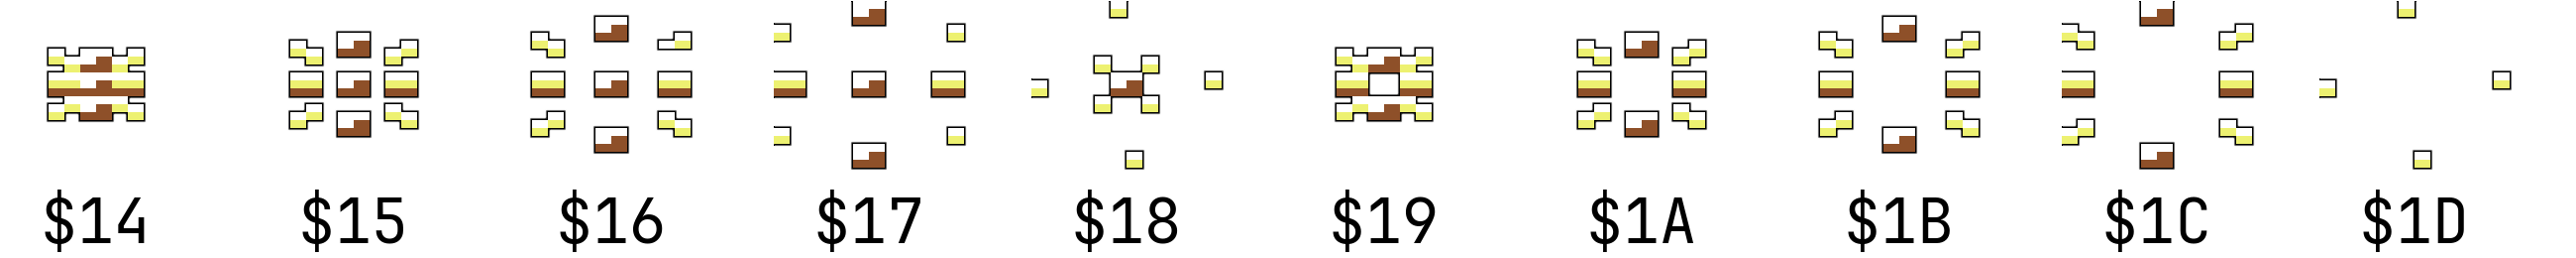
\includegraphics{src/enemy_bullets/level9_explosion_sequence.png}%
  \end{adjustbox}
\end{figure}
\vspace{-0.4cm}

As with the uridimine, the composited sequence of the explosion shows us how the overall effect
is of spokes radiating from a single source - something not immediately obvious when the members
of the sequence are displayed side by side. This explosion is the end of the bullet's lifecycle
(as you might expect). Notice how our final act is to free up a slot in \fcode{indexToEnemyUpdatePtrArray}
by writing zero to it and decrementing \fcode{bulletsInProgress} to update the number of bullets
currently active.

\vspace{-0.2cm}
\begin{minipage}[c]{0.30\linewidth}
	\vspace{-0.1cm}
	\begin{figure}[H]
		\centering
		\begin{adjustbox}{width=4.0cm,center}
			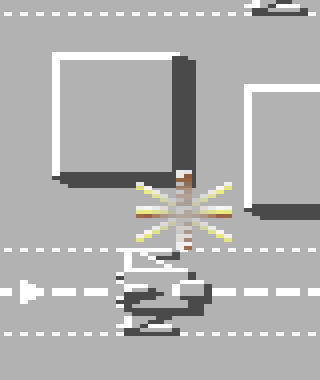
\includegraphics{src/enemy_bullets/level9_bullet_explodes.png}%
		\end{adjustbox}
	\end{figure}
\end{minipage}
\begin{minipage}[c]{0.68\linewidth}
\begin{lstlisting}[basicstyle=\scriptsize\ttfamily]
AnimateEnemyExplosion
  JSR FollowMantaOnX      ; Follow Manta along X axis.
  LDA frameRate           ; Check the frame rate.
  AND #$01                ; Make it between 0 and 1.
  BNE DetectLeavingScreen 
  INC currentSpriteValue  ; Move to next sprite.
  LDA currentSpriteValue  ; Check progress..
  CMP #$1E                ; If it's reached $1E then..
  BCC DetectLeavingScreen ; .. we're finished launching.
  LDA #$00                ; Put $00 in A.
  STA spriteEnable        ; Disable the sprite.
  LDY currentEnemyIndex   ; Get the mine's index.
  STA indexToEnemyUpdatePtrArray,Y ; Store 0 in function.
  DEC bulletsInProgress   ; Free up a slot.
  JSR DisplayCurrentSprite ; Display erased sprite.
  RTS
\end{lstlisting}
\end{minipage}
